%File: formatting-instruction.tex
\documentclass[letterpaper]{article}
% AAAI format packages
\usepackage{aaai}
\usepackage{times}
\usepackage{helvet}
\usepackage{courier}
% Additional packages
\usepackage{amsmath}
\usepackage{amssymb}
\usepackage{amsthm}
\usepackage{algorithm}
\usepackage{algorithmic}
\usepackage{graphicx}
\usepackage{comment}
\newtheorem{defn}{Definition}
\newtheorem{lemma}{Lemma}
\newtheorem{thm}{Theorem}
\newtheorem{cor}{Corollary}
\newtheorem{rul}{Expansion Rule}
% END Additional packages
\frenchspacing
\setlength{\pdfpagewidth}{8.5in}
\setlength{\pdfpageheight}{11in}
\pdfinfo{
/Title (Enhanced Parallel A* for Slow Expansions)
%/Author (Aram Ebtekar, Mike Phillips, Sven Koenig, Maxim Likhachev)
/Keywords (weighted A* search, parallel algorithm, heuristic)
}
\setcounter{secnumdepth}{0}  
 \begin{document}
% The file aaai.sty is the style file for AAAI Press 
% proceedings, working notes, and technical reports.
%
\title{Enhanced Parallel A* for Slow Expansions}
\author{Aram Ebtekar$^\dagger$ \and Mike Phillips$^\dagger$ \and Sven Koenig\thanks{University of Southern California, Los Angeles, CA 90089} \and Maxim Likhachev% <-this % stops a space
\thanks{Carnegie Mellon University, Pittsburgh, PA 15217}% <-this % stops a space
%
}
\author{AAAI 2015 Submission 2327}% anonymizer
\maketitle
\begin{abstract}
\begin{quote}
In order for heuristic searches to take advantage of modern CPU architectures, the algorithms must be parellelized.
wPA*SE is a recent parallel variant of A*, which expands each state at most once and guarantees a solution cost not exceeding a specified factor of the optimal.
wPA*SE can achieve a nearly linear speedup in the number of processor cores if expansions are sufficiently time-consuming to dominate the search runtime.
Much of the overhead of wPA*SE is due to careful selection of states to expand, as required to meet the theoretical guarantees.
In this work, we present extensions to wPA*SE that maintain speedups at faster expansion rates than wPA*SE allows.
They reduce the overhead of selecting states for expansion by maintaining tighter bounds on the suboptimality of each state.
On the theoretical side, we provide the same guarantees on completeness and solution quality as wPA*SE.
Experimentally, we show comparable performance to wPA*SE when expansions are slow, and better performance as expansions become faster and the number of cores increases.
Finally, we present an extension to the anytime setting.
\end{quote}
\end{abstract}

\begin{algorithm}
\caption{$update(s)$}
\label{alg:update}
\begin{algorithmic}
\STATE $bp(s) := \arg\min_{s'} v(s') + c(s',s)$
\STATE $g(s) := v(bp(s)) + c(bp(s),s)$
\STATE $g_p(s) := \min_{s'\in CLOSED} bound(s') + \epsilon c(s',s)$
\IF{$v(s) > g(s)$}
\IF{$s\in CLOSED$}
\STATE move $s$ to $FROZEN$
\ELSE
\STATE move $s$ to $OPEN^+$
\ENDIF
\ELSIF{$v(s) < g(s)$}
\STATE move $s$ to $OPEN^-$
\ELSE
\STATE remove $s$ from $OPEN^+$, $OPEN^-$, $FROZEN$
\ENDIF
\end{algorithmic}
\end{algorithm}

\begin{algorithm}
\caption{$main()$}
\label{alg:main}
\begin{algorithmic}
\STATE $OPEN := BE := CLOSED := FROZEN := \emptyset$
\STATE $g(s_{start}) := 0$
\STATE $expand(s_{start})$
\REPEAT
\FORALL{changed edges $(u,v)$}
\STATE $update(v)$
\ENDFOR
\STATE $thaw()$
\STATE $search()$ on multiple threads in parallel
\UNTIL{done}
\end{algorithmic}
\end{algorithm}

\begin{algorithm}
\caption{$search()$}
\label{alg:search}
\begin{algorithmic}
\WHILE{$g(s_{goal}) > bound(s_{goal})$}
\STATE remove any $s\in OPEN^+\cup OPEN^-$ and LOCK $s$
\IF{$safe(s)$}
\STATE insert $s$ into $CLOSED$
\IF{$v(s)\le bound(s)$}
\STATE insert $s$ into $FROZEN$
\STATE continue
\ENDIF
\ENDIF
\STATE insert $s$ into $BE$ with key $f(s)$
\STATE $v_{expand} := g(s)$
\STATE UNLOCK $s$
\STATE $expand(s)$
\STATE $v(s) := v_{expand}$
\STATE remove $s$ from $BE$
\ENDWHILE
\end{algorithmic}
\end{algorithm}

\begin{algorithm}
\caption{$expand(s)$}
\label{alg:expand}
\begin{algorithmic}
\FORALL{$s' \in successors(s)$}
\STATE LOCK $s'$
\IF{$s'$ has not been generated yet}
\STATE $g(s') := v(s') := g_p(s') := \infty$
\ENDIF
\IF{$s\in CLOSED$ \AND $g_p(s') > bound(s) + \epsilon c(s,s')$}
\STATE $g_p(s') = bound(s) + \epsilon c(s,s')$
\ENDIF
\IF {$g(s') > g(s) + c(s,s')$}
\STATE $g(s') := g(s) + c(s,s')$
\STATE $bp(s') := s$
\IF{$s' \in CLOSED$}
\STATE insert $s'$ in $FROZEN$
\ELSE
\STATE insert/update $s'$ in $OPEN^+$/$OPEN^-$ with key $f(s')$
\ENDIF
\ENDIF
\STATE UNLOCK $s'$
\ENDFOR
\end{algorithmic}
\end{algorithm}

\begin{algorithm}
\caption{Auxiliary Functions}
\label{alg:aux}
\begin{algorithmic}
\STATE \textbf{FUNCTION} $successors(s)$
\RETURN $\{s' \mid c(s,s')<\infty\}$

\STATE \textbf{FUNCTION} $f(s)$
\IF{$g(s) < v(s)$}
\RETURN $g(s) + wh(s,s_{goal})$
\ELSE
\RETURN $v(s) + h(s,s_{goal})$
\ENDIF
\end{algorithmic}
\end{algorithm}

\begin{algorithm}
\caption{$bound(s)$ enhanced for ePA*SE/PARA*}
\label{alg:eaux}
\begin{algorithmic}
\STATE \textbf{FUNCTION} $g_{back}(s',s)$
\IF{$s' = NULL$}
\RETURN $\infty$
\ELSIF{$w \le \epsilon$}
\RETURN $g(s) + f(s') - f(s) + (2\epsilon-w-1)c_l$
\ELSE
\RETURN $\frac\epsilon w\left(g(s) + f(s') - f(s)\right) + (\epsilon-1)c_l$
\ENDIF

\STATE \textbf{FUNCTION} $v_{back}(s',s)$
\IF{$s' = NULL$}
\RETURN $\infty$
\ELSE
\RETURN $v(s) + f(s') - f(s)$
\ENDIF

\STATE \textbf{FUNCTION} $vbound(s)$
\STATE $v_{front} := \infty$
\STATE $s' :=$ first state in $OPEN^-\cup BE^-$
\WHILE{$v_{back}(s',s) \le g(s) < v_{front}$}
\STATE $v_{front} := \min(v_{front},\;v(s') + h(s',s))$
\STATE $s' :=$ state following $s'$ in $OPEN^-\cup BE^-$
\ENDWHILE
\RETURN $\min(v_{front},\;v_{back}(s',s))$

\STATE \textbf{FUNCTION} $bounded(s)$
\STATE $g_{front} := g_p(s)$
\STATE $s' :=$ first state in $OPEN^+ \cup BE^+$
\WHILE{$g_{back}(s',s) < g(s) \le g_{front}$}
\STATE $g_{front} := \min(g_{front},\;g_p(s') + \epsilon h(s',s))$
\STATE $s' :=$ state following $s'$ in $OPEN^+ \cup BE^+$
\ENDWHILE
\STATE $bound(s) := \max\left(bound(s), \; \min(g_{front},\;g_{back}(s',s))\right)$
\RETURN $g(s) \le bound(s)$ \AND $g(s) < vbound(s)$
\end{algorithmic}
\end{algorithm}

\begin{algorithm}
\caption{$thaw()$}
\label{alg:thaw}
\begin{algorithmic}
\STATE choose new $\epsilon \in [1,\infty]$ and $w \in [0,\infty]$
\STATE $OPEN := OPEN \cup FROZEN$ with keys $f(s)$
\STATE $CLOSED := FROZEN := \emptyset$
\FORALL{$s\in OPEN$}
\STATE $g_p(s) := g(s) + (\epsilon-1)\min(g(s),\;2c_l)$
\ENDFOR
\end{algorithmic}
\end{algorithm}

The following lemma lists some easily checked invariants of ePA*SE and PARA*.

\begin{lemma}
\label{lem:prop}
At all times, the following invariants hold:
\begin{itemize}
\item $OPEN\cap CLOSED = \emptyset$
\item $BE\cup FROZEN \subseteq CLOSED$
\item If $g(s)<\infty$, $bp(\cdot)$ can be followed from $s$ back to $s_{start}$ to yield a path from $s_{start}$ to $s$ costing at most $g(s)$
\item If $s\ne s_{start}$, then $g(s) + (\epsilon-1)c_l \le g_p(s)$,
\\$g_p(s) \le min_{s'\in CLOSED}\left\{\epsilon (g^*(s') + c(s',s))\right\}$, and
\\$g(bp(s)) + c(bp(s),s) \le g(s) \le min_{s'}\left\{v(s') + c(s',s)\right\}$
\item $g(s) < v(s) \Leftrightarrow s\in OPEN^+\cup BE^+\cup FROZEN$
\item $g(s) > v(s) \Leftrightarrow s\in OPEN^-\cup BE^-$
\item $s\in OPEN\cup CLOSED$ iff we had $g(s)<v(s)$ sometime since the most recent call to $thaw()$
\end{itemize}
\end{lemma}

\begin{proof}
Induction on time.
\end{proof}

The last line of the fourth point is a relaxation of $g(s) = \min_{s'}\{v(s') + c(s',s)\}$, an invariant often seen in sequential A* variants such as ARA*. Our relaxation allows more parallel variable assignments, such as modifying the $g$-value of a state which is undergoing expansion.

\begin{rul}
We can expand $s\in REPAIR$ freely and move it to $OPEN$, though we should prefer to take the front element. We can expand $s\in OPEN$ freely as well, but can only put it in $CLOSED$ if $g(s) \le bound(s)$ and $g(s) < vbound(s)$.
\end{rul}

\section{Theoretical Analysis}

\subsection{Correctness}

We investigate ePA*SE/PARA* beginning at the core: the $bound$ function of Algorithm \ref{alg:eaux}.

\begin{lemma}
\label{lem:indep}
At all times, for all states $s$ and $s'\notin \{s_{start},s\}$:
\[g_{back}(s',s) \le g_p(s') + \epsilon h(s',s).\]
\end{lemma}

\begin{proof}
If $w \le \epsilon$, then
\begin{eqnarray*}
&&g(s) + f(s') - f(s) + (2\epsilon-w-1)c_l
\\&=& g(s') + w(h(s',s_{goal}) - h(s,s_{goal})) + (2\epsilon-w-1)c_l
\\&\le& g(s') + wh(s',s) + (2\epsilon-w-1)c_l
\\&\le& g(s') + \epsilon h(s',s) + (w-\epsilon)c_l + (2\epsilon-w-1)c_l
\\&=& g(s') + (\epsilon-1)c_l + \epsilon h(s',s)
\\&\le& g_p(s') + \epsilon h(s',s)
\end{eqnarray*}
where the last two inequalities follow by WLOG having $h(s,s') \ge c_l$ and Lemma \ref{lem:prop}.

On the other hand, if $w > \epsilon$, then
\begin{eqnarray*}
&&\frac\epsilon w\left(g(s) + f(s') - f(s)\right) + (\epsilon-1)c_l
\\&=& \frac\epsilon w\left(g(s') + w(h(s',s_{goal}) - h(s,s_{goal})) \right) + (\epsilon-1)c_l
\\&\le& g(s') + \epsilon(h(s',s_{goal}) - h(s,s_{goal})) + (\epsilon-1)c_l
\\&\le& g(s') + (\epsilon-1)c_l + \epsilon h(s',s)
\\&\le& g_p(s') + \epsilon h(s',s)
\end{eqnarray*}
\end{proof}

\begin{lemma}
\label{lem:bound}
For every state $s$,
\[bound(s) \le \min_{s'\in OPEN \cup BE} \left\{ g_p(s') + \epsilon h(s',s) \right\}.\]
Furthermore, $g(s) \le bound(s)$ iff
\[g(s) \le \min_{s'\in OPEN \cup BE} \left\{ g_p(s') + \epsilon h(s',s) \right\}.\]
\end{lemma}

\begin{proof}
By construction, $g_{front}$ is bounded above by $g_p(s') + \epsilon h(s',s)$ for all $s'\in V$, where $V$ consists of $s$ and the states considered by the loop in $bound(s)$. Meanwhile, Lemma \ref{lem:indep} ensures that $g_{back}$ is bounded above by $g_p(s') + \epsilon h(s',s)$ for all $s'\in \bar V$, where $\bar V = (OPEN \cup BE) \setminus V$. Therefore,
\[bound(s) \le \min_{s' \in OPEN \cup BE} \left\{g_p(s') + \epsilon h(s',s)\right\}.\]
To prove the second claim, note that the loop in $bound(s)$ terminates under one of two conditions.

If the loop terminates because $g(s) \le g_{back}$, then by Lemma \ref{lem:indep}, $g(s) \le g_{back} \le \min_{s'\in \bar V} \left\{ g_p(s') + \epsilon h(s',s) \right\}$. Since $g_{front} = \min_{s'\in V} \left\{ g_p(s') + \epsilon h(s',s) \right\}$, it follows that $g(s) \le bound(s)$ iff $g(s) \le \min_{s'\in OPEN \cup BE} \left\{ g_p(s') + \epsilon h(s',s) \right\}$.

On the other hand, if the loop terminates because $g(s) > g_{front}$, then the final assignment to $g_{front}$ must correspond to a state $s'$ for which
\[g(s) > g_p(s') + \epsilon h(s',s) = g_{front} \ge bound(s).\]
\end{proof}

\begin{thm}
\label{thm:subopt}
For all $s\in OPEN\cup BE$, $bound(s) \le \epsilon g^*(s)$. Hence, for all $s\in CLOSED$, $g(s) \le v(s) \le \epsilon g^*(s)$.
\end{thm}

\begin{proof}
We proceed by induction on the order in which states are expanded.

Let $\pi = \langle s_0,s_1,\ldots,s_N \rangle$ be a minimum-cost path from $s_0 = s_{start}$ to $s_N = s\in OPEN\cup BE$. Choose the minimum $i$ such that $s_i\in OPEN\cup BE$. If $i = 1$, then since $s_0 = s_{start}$ was already expanded,
\[g_p(s_1) \le \epsilon c(s_0,s_1) = \epsilon g^*(s_1).\]
If $i \ge 2$, there are two cases to consider, depending on whether $s_{i-1}\in CLOSED$.

If so, the induction hypothesis implies $v(s_{i-1}) \le \epsilon g^*(s_{i-1})$. Hence by Lemma \ref{lem:prop},
\begin{eqnarray*}
g_p(s_i) &\le& v(s_{i-1}) + \epsilon c(s_{i-1},s_i)
\\&\le& \epsilon g^*(s_{i-1}) + \epsilon c(s_{i-1},s_i)
\\&=& \epsilon g^*(s_i)
\end{eqnarray*}

On the other hand, suppose $s_{i-1}\notin CLOSED$, as might occur after a $thaw()$. Choose the maximum $j<i$ such that $s_j\in CLOSED$, or $j=0$ if there is no such $j$. Then $j\le i-2$ so $c^*(s_j,s_i)\ge 2c_l$ and, by the induction hypothesis, $v(s_j)\le \epsilon g^*(s_j)$.

Let $g_{old}(s_i)$ denote the value of $g(s_i)$ at the time of the most recent $thaw()$ (or $\infty$ is no $thaw()$ has occurred). For all $j < k < i$, $s_k$ can never have been in $OPEN\cup CLOSED$ after the last $thaw()$; for if it had, then it would remain in $OPEN\cup CLOSED$, in contradiction to our construction of $i$ and $j$. Thus, Lemma \ref{lem:prop} implies $g(s_k) = v(s_k)$ held ever since the last $thaw()$, and so $g_{old}(s_i) \le v(s_j) + c^*(s_j,s_i)$. Now by the initialization of $g_p$,
\begin{eqnarray*}
g_p(s_i) &\le& g_{old}(s_i) + 2(\epsilon-1)c_l
\\&\le& v(s_j) + c^*(s_j,s_i) + 2(\epsilon-1)c_l
\\&\le& \epsilon g^*(s_j) + c^*(s_j,s_i) + 2(\epsilon-1)c_l
\\&=& \epsilon (g^*(s_j) + c^*(s_j,s_i)) + (\epsilon-1)(2c_l - c^*(s_j,s_i))
\\&\le& \epsilon g^*(s_i)
\end{eqnarray*}

In all three cases, we see that
\[g_p(s_i) + \epsilon h(s_i,s) \le \epsilon g^*(s_i) + \epsilon c^*(s_i,s) = \epsilon g^*(s).\]

Therefore, by Lemma \ref{lem:bound},
\[bound(s) \le \min_{s' \in OPEN \cup BE} \left\{g_p(s') + \epsilon h(s',s)\right\} \le \epsilon g^*(s).\]
\end{proof}

\begin{cor}
\label{cor:subopt}
At the end of ePA*SE or a search round of PARA*, the path obtained by following the back-pointers $bp(\cdot)$ from $s_{goal}$ to $s_{start}$ is an $\epsilon$-suboptimal solution.
\end{cor}

\begin{proof}
The termination condition of the search is $g(s_{goal}) \le bound(s_{goal})$. By construction, the path given by following back-pointers costs at most $g(s_{goal})$. The claim now follows from Theorem \ref{thm:subopt}.
\end{proof}

\subsection{Completeness}

Having shown correctness of the algorithm at termination, it only remains to show that ePA*SE and every search round of PARA* indeed terminates. This is trivial on finite graphs, but we can also say something about a class of infinite graphs. The proof appears in the extended version of this paper.

\begin{thm}
\label{thm:complete}
ePA*SE and the search rounds of PARA* terminate in finite time, provided $w$, $g^*(s_{goal})$ and the out-degrees of states are all finite, and $c_l > 0$.
\end{thm}

\begin{proof}

Let $\pi = \langle s_0,s_1,\ldots,s_N \rangle$ be a minimum-cost path from $s_0 = s_{start}$ to $s_N = s_{goal}$. At any fixed time in the algorithm's operation, let $i$ be maximal such that $g(s_i)<\infty$ and $g(s_i)\le\epsilon g^*(s_i)$. We will prove that $s_i$ is eventually expanded. Since expanding $s_i$ ensures $g(s_{i+1})\le \epsilon g^*(s_i)+c(s_i,s_{i+1})\le\epsilon g^*(s_{i+1})$, it then follows by mathematical induction that $g(s_{goal})$ eventually attains a finite value not exceeding $\epsilon g^*(s_{goal})$.

First, suppose for contradiction that $v(s_i)\le \epsilon g^*(s_i)$. Then by Lemma \ref{lem:prop}, $g(s_{i+1}) \le v(s_i)+c(s_i,s_{i+1})\le\epsilon g^*(s_i)+c(s_i,s_{i+1})\le\epsilon g^*(s_{i+1})$, in contradiction to our construction of $i$. Thus, we must have $g(s_i)\le\epsilon g^*(s_i)<v(s_i)$, which by Lemma \ref{lem:prop} and Theorem \ref{thm:subopt} implies $s_i\in OPEN$. Let $\alpha = \min(w,\epsilon)$ and
\[C = \frac w\alpha \left( v(s_i) + c(s_i, s_{i+1}) \right) + wh(s_{i+1}, s_N).\]

Once $s_i$ is expanded, $C$ is hereafter a constant. If we define $f_\alpha(s) = g(s) + \alpha h(s)$ and fix an $s\in OPEN\cup BE$ with minimum $f_\alpha$-value, then $s$ is safe for expansion. Now, $f(s) \le \frac w\alpha f_\alpha(s) \le \frac w\alpha f_\alpha(s_i) \le C$. Consider the set of states with $f$-value at most $C$. Since $s$ is safe for expansion, and states in $OPEN\cup BE$ are considered in order of increasing $f$, it must be the case that either some state in this set is currently being expanded,  or the next state to be selected for expansion will be in this set. To show that $s_i$ is eventually expanded, it now suffices to show that this set is finite.

Each edge costs at least $c_l$, so any state $s$ which is separated from $s_{start}$ by more than $C/c_l$ edges must have $f(s) \ge g(s) > C$. Having bounded the depth at which the set of states $s$ satisfying $f(s) \le C$ may appear, finite out-degrees imply this set must have finite size.

To summarize, in finite time we obtain $f(s_{goal}) = g(s_{goal}) \le \epsilon g^*(s_{goal})$. By a similar argument to the above, it follows that only finite time can take place before $s_{goal}$ becomes safe for expansion, and the latter criterion is precisely the search termination condition.
\end{proof}

\subsection{Asymptotic Time Complexity}

To get a sense for the increased parallelism of ePA*SE, we analyze its worst-case time complexity in the limit where an unbounded supply of processors are available, the goal state is far from the start, and $w \le \epsilon$. To simplify matters, we consider a ``blind" version of ePA*SE which considers only the frontmost state $s\in OPEN$ and in which, if the while loop condition of Algorithm \ref{alg:eaux} succeeds, $s$ is immediately deemed unsafe for expansion. This effectively removes the while loop. 

If $|OPEN|$ is the frontier size, $|BE|$ is the number of states deemed simultaneously safe for expansion, and $D$ is the maximum out-degree of a state, then having each of $|BE|$ threads simultanously expand one node from the frontier now takes $O\left((|BE|+D)\log|OPEN|\right)$ time. Since any state deemed safe by Blind ePA*SE can be extracted just as quickly by ePA*SE, any performance guarantees we prove here will also apply to ePA*SE and PARA*.

Let one \textbf{parallel expansion time (PET) unit} be the time needed for all threads to simultaneously extract and expand one state, unless the blind safety check fails in which case they expand nothing. Algorithm \ref{alg:eaux} (and its blind variant) declares all states with $f$-value deviating by no more than $(2\epsilon-w-1)c_l$ safe for expansion, so they are all expanded in a single PET. In such a setting, the following bound applies:

\begin{thm}
\label{thm:depth}
If $w \le 1$, ePA*SE completes in at most
\[\min\left(\frac{\epsilon g^*(s_{goal})}{(1-w)c_l},\;
\frac{\left(\epsilon g^*(s_{goal})\right)^2 + O(g^*(s_{goal})) }{(4\epsilon-2w-2)c_l^2} \right)\text{ PETs.}\]
\end{thm}

\begin{proof}
We prove the two bounds separately. For the first, note that if the minimum $f$-value is $f_{min}$, every state with $f$-value up to $f_{min} + (2\epsilon-w-1)c_l$ can be expanded simultaneously. Since $h$ is consistent, the successors' $f$-values are at least $f_{min} + (1-w)c_l$. Hence, one PET increases $f_{min}$ by at least $(1-w)c_l$. When $s_{goal}$ is expanded, $f(s_{goal}) = g(s_{goal}) \le \epsilon g^*(s_{goal})$. Since $f_{min}$ is initially $f(s_{start}) = h(s_{start}) \ge 0$, it suffices to take
\[\frac{\epsilon g^*(s_{goal})}{(1-w)c_l}\text{ PETs.}\]

For the other bound, let $t=2\epsilon-w-1$. Since $f$-values never decrease along paths, once the minimum $f$-value in $OPEN$ surpasses $f_{min}$, from then on all states with $f$-value up to $f_{min} + tc_l$ are always safe for expansion.

With each subsequent time step, states with $f$-value up to $f_{min} + tc_l$ have their $g$-values increased by at least $c_l$. Since $g$ cannot exceed $f$, this continues for at most $(f_{min} + tc_l) / c_l = f_{min}/c_l + t$ iterations, after which every state in $OPEN$ has $f$-value $\ge f_{min} + tc_l$. Continuing this process until $f_{min}$ exceeds $\epsilon g^*(s_{goal})$, the total number of PETs required is at most
\begin{eqnarray*}
&&t + 2t + 3t + \ldots + \lfloor u+1 \rfloor t
\\&\le& \frac t2 (u+1)(u+2)
\\&=& \frac t2 (u^2 + O(u))
\\\text{where }u &=& \frac{\epsilon g^*(s_{goal})}{c_lt}.
\end{eqnarray*}
\end{proof}

Thus, if we ignore factors hidden in the PET unit, the worst-case time complexity of ePA*SE is roughly linear in the goal distance when $w$ is considerably smaller than 1, and becomes quadratic as $w \rightarrow 1$. Compare this against the exponential complexity of sequential search. This result suggests that using $w < \epsilon$ might become favorable as upcoming technological developments raise the supply of processor cores. The case $w = 0$ completely ignores the heuristic-to-goal, yielding a parallel anytime algorithm for the classic  single-source shortest paths problem.

Finally, the case $w > \epsilon$ merits future investigation as it allows a greedier bias in the frontier ordering, without loosening the suboptimality guarantee. While we de not recommend it in practice as it demands extensive checking during state extraction, it may be worthwhile if expansion times are especially long. Furthermore, we gain usable information from the additional checks, as the tightened result of $bound(s)$ propagates via $g_p$. The $w = \infty$ extreme corresponds to sorting by $h$-value. Indeed, if we are willing to check against all of $OPEN\cup BE$, then arbitrary orderings on $OPEN$ and $BE$ become permissible, but at the price of the completeness promised by Theorem \ref{thm:complete}.

Finally, suppose that in place of the minimum cost $c_l$, we are given an estimate $c_m$ of the mean edge cost along a solution. Taking inspiration from \cite{klein1997randomized}, we ``grow" the small edges by a length not exceeding $\delta = (\alpha-1)c_m$ where $\alpha$ is the desired suboptimality bound. We then run ePA*SE with the bound $c_l' = c_l+\delta$, costs $c'(s,s') = \max(c(s,s'), c_l')$, and heuristic $h'(s,s') = \max(h(s,s'), c_l')$. The resulting search satisfies a bound analoguous to Theorem \ref{thm:depth}, even if $c_l=0$.

\begin{thm}
\label{thm:delta}
If the mean cost of the edges along a minimum-cost path to $s$ is at least $c_m$, then upon expansion, $g'(s) \le \epsilon(1+\delta/c_m)g^*(s)$. Therefore, to achieve a suboptimality factor $\alpha$, we can set $\epsilon=1$ and $\delta = (\alpha-1)c_m$.
\end{thm}

\begin{proof}
Let $k(s)$ be the number of edges along a minimum-cost path to $s$. We assumed $g^*(s) / k(s) \ge c_m$, so $k(s) \le g^*(s) / c_m$.
Since edge costs were increased by at most $\delta$, Theorem \ref{thm:subopt} implies $g'(s) \le \epsilon g'^*(s) \le \epsilon(g^*(s) + \delta k(s)) \le \epsilon(1+\delta/c_m)g^*(s)$. Furthermore, since no edge cost was decreased, any path found on the modified graph costs no more on the original graph.
\end{proof}

\begin{cor}
\label{cor:delta}
If $w \le 1$ and $c_m \le g^*(s_{goal}) / k(s_{goal})$, ePA*SE can be used to find an $\alpha$-optimal solution in at most
\[\frac{\alpha g^*(s_{goal})}{(1-w)(c_l+(\alpha-1)c_m)}\text{ PETs.}\]
If, in addition, $c_m \ge g^*(s_{goal})/(mk(s_{goal}))$, this method takes at most
\[\frac{\alpha mk(s_{goal})}{(1-w)(\alpha-1)}\text{ PETs.}\]
\end{cor}

In other words, if $\alpha$ is far from $1$ and we know the mean edge cost up to a small constant factor, we can find approximately optimal paths within a small time factor of the ``omnicient" algorithm that expands only along the optimal path.

\section{Experiments}

We tested wPA*SE and ePA*SE with parameters $w=\epsilon=1.5$ on a 2D grid domain with 8-connected cells. We used the same 20 maps as \cite{phillips2014pa} from a commonly used pathfinding benchmark \cite{sturtevant2012benchmarks}. The searches were run on an Amazon EC2 machine with a 32-core Intel Xeon E5-2680v2.

In the first set of experiments, we varied the time per expansion between $10^{-6}$, $10^{-5}$ and $10^{-4}$ seconds, and the number of threads between 1, 2, 4, 8, 16, 24 and 32. For each of these settings, Figure \ref{fig:time} displays the average speedup factor: the time taken by a sequential wA* search divided by the time taken by wPA*SE or ePA*SE. We observe moderate gains over wPA*SE as the number of cores increases, especially when expansion times are fairly fast. However, although ePA*SE demonstrates greater parallelism than wPA*SE, both algorithms falter when the number of threads is too high. This seems to be due to the fact that the data structure locks ensure only one thread can work on state extraction at a time. If the number of threads is high, some expansions finish before a new state is extracted, so the threads never become saturated, resulting in needless overhead. To achieve greater parallelism, it may become necessary to parallelize the extraction process so that multiple threads can access the frontier simultaneously.

In the second set of experiments, we varied the time per expansion between $10^{-5}$ and $10^{-4}$ seconds, and the weight parameters $w=\epsilon$ between 1.1, 1,5, 2, 3 and 4. Figure \ref{fig:eps} displays the speedup factor for each setting in a similar format. We observe that ePA*SE achieves very high gains when the weight is low, gradually dissipating as the weight increases. In particular, when the weight is close to 1, the speedup over sequential search is approximately linear in the number of processors. ePA*SE is found to perform at least as well as the tested competitors in all cases, and considerably better in some classes of scenarios.

\begin{figure}[fig:time]
\centering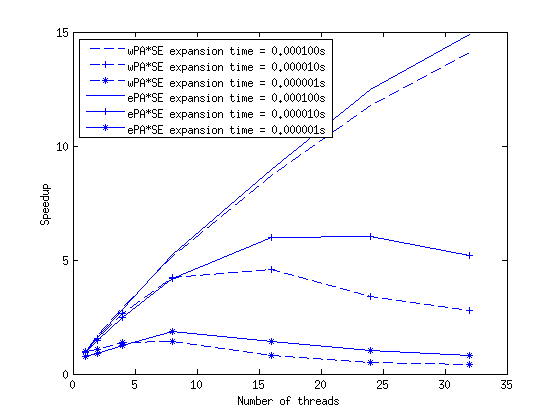
\includegraphics[scale=0.55]{time_sweep_para.png}
\caption{2D grid speedup as the number of threads and expansion time are varied.}
\end{figure}

\begin{figure}[fig:tps]
\centering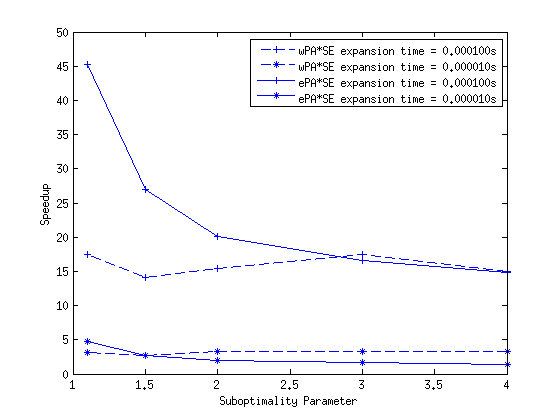
\includegraphics[scale=0.55]{eps_sweep_para.png}
\caption{2D grid speedup as the weight parameter and expansion time are varied.}
\end{figure}

\section{Conclusion}

We have presented a framework which unifies wA* and wPA*SE, differentiating them primarily by expansion rule. Within this framework, we created ePA*SE and proved it maintains the completeness and guaranteed bounded suboptimality of wPA*SE, with additional performance bounds in the limit of massive parallelism. We showed experimental gains in performance, presented an anytime variant, and discussed the role of decoupling the weight parameter from the suboptimality factor.

Future work remains to experimentally investigate the effect of using $w \ne \epsilon$ under various settings. The bottleneck of ePA*SE appears to be the fact that only one thread at a time can access the data structures to extract states. While prior work includes techniques for splitting the frontier for parallel access, none so far have all the theoretical benefits we showed for ePA*SE.

\bibliographystyle{aaai}
\bibliography{epase}

\end{document}
